\FILENAME

\section{GrovePi Modules}\label{grovepi-modules}

\subsection{Intro}\label{intro}

\begin{itemize}
\tightlist
\item
  \href{http://www.instructables.com/id/Basic-Electronics}{Electronics}:
  An introduction to the basic principals of electronics.
\item
  \href{https://learn.sparkfun.com/tutorials/voltage-current-resistance-and-ohms-law}{Volatage}:
  An introduction to the physics of electricity.
\item
  \href{https://info-ee.eps.surrey.ac.uk/Teaching/Unix/index.html}{Unix}:
  An introduction to the Unix os.
\item
  \href{https://github.com/DexterInd/GrovePi/tree/master/Software/Python}{grove
  examples}: A list of Dexter Industries example code for GrovePi
  modules.
\item
  \href{https://github.com/cloudmesh/cloudmesh.pi/tree/master/cloudmesh/pi}{GrovePi
  module classes}: A repository for the GrovePi module classes.
\end{itemize}

\subsection{LED}\label{led}

An LED is the simplest possible module for a raspberry pi, as it is
responsive only to the provided power. For an LED to emit light, it must
be exposed to a voltage greater than a certain threshold value. Above
this voltage, the conductivity of the diode increases exponentially and
its brightness increases likewise. If the current through the LED
becomes too high, the LED will burn out. The following link leads to a
tutorial from Dexter Industries for the LED module.

\begin{itemize}
\tightlist
\item
  \href{https://www.dexterindustries.com/GrovePi/projects-for-the-raspberry-pi/raspberry-pi-led-tutorial/}{Dexter
  LED tutorial}
\end{itemize}

Connect the LED To a digital port. The following code describes an LED
class. Since it is connected to a digital output, the voltage has only
two states, on and off. The default port for the LED class is D3. The
code for the \texttt{LED} class can be found here:

\begin{itemize}
\tightlist
\item
  \href{https://github.com/cloudmesh/cloudmesh.pi/blob/master/cloudmesh/pi/led.py}{LED
  Class}
\end{itemize}

\begin{figure}
\centering
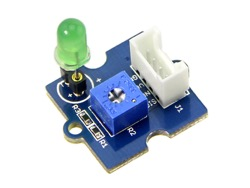
\includegraphics{../images/grovepi/led.jpg}
\caption{LED}
\end{figure}

\subsection{Buzzer}\label{buzzer}

Connect the buzzer to a digital port. The default port for the Buzzer
class is D3. You will notice that the Buzzer class and the LED class are
interchangeable. This is because they work on the same digital
principal. Their two values are on and off. The code for the
\texttt{Buzzer} class can be found here:

\begin{itemize}
\tightlist
\item
  \href{https://github.com/cloudmesh/cloudmesh.pi/blob/master/cloudmesh/pi/buzzer.py}{Buzzer
  Class}
\end{itemize}

\begin{figure}
\centering
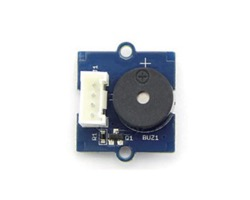
\includegraphics{../images/grovepi/buzzer.jpg}
\caption{Buzzer}
\end{figure}

\subsection{Relay}\label{relay}

The relay acts as a switch in a circuit. When the value on the relay is
1, it allows current to flow through it. When the value is 0, the relay
breaks the circuit and the current stops. Connect the relay to a digital
port. The default digital port is D4. The \texttt{Relay} class can be
found here:

\begin{itemize}
\tightlist
\item
  \href{https://github.com/cloudmesh/cloudmesh.pi/blob/master/cloudmesh/pi/relay.py}{Relay
  Class}
\end{itemize}

\begin{figure}
\centering
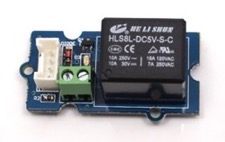
\includegraphics{../images/grovepi/relay.jpg}
\caption{Relay}
\end{figure}

\subsection{Light Sensor}\label{light-sensor}

The light sensor measures ligh intensity and returns a value between 0
and 1023. Connect the light sensor to an analog port. The default port
is A0. The analog port allows the light sensor to return a range of
values. The \texttt{LightSensor} class can be found here:

\begin{itemize}
\tightlist
\item
  \href{https://github.com/cloudmesh/cloudmesh.pi/blob/master/cloudmesh/pi/light.py}{LightSensor
  Class}
\end{itemize}

\begin{figure}
\centering
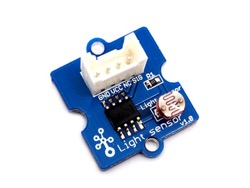
\includegraphics{../images/grovepi/light.jpg}
\caption{Light Sensor}
\end{figure}

\subsection{Rotary Angle Sensor}\label{rotary-angle-sensor}

The rotary angle sensor measures the angle to which it is turned.
Connect the sensor to an analog port. Port A0 is the default. The
\texttt{RotarySensor} class can be found here:

\begin{itemize}
\tightlist
\item
  \href{https://github.com/cloudmesh/cloudmesh.pi/blob/master/cloudmesh/pi/rotary.py}{RotarySensor
  Class}
\end{itemize}

\begin{figure}
\centering
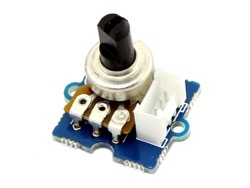
\includegraphics{../images/grovepi/rotary.jpg}
\caption{Rotary Angle Sensor}
\end{figure}

\subsection{Barometer}\label{barometer}

Connect the barometer to an I2C port. In addition to pressure, the
GrovePi barometer measures temperature in Fahrenheit and Celcius. The
\texttt{Barometer} class can be found here.

\begin{itemize}
\tightlist
\item
  \href{https://github.com/cloudmesh/cloudmesh.pi/blob/master/cloudmesh/pi/barometer.py}{Barometer
  Class}
\end{itemize}

\begin{figure}
\centering
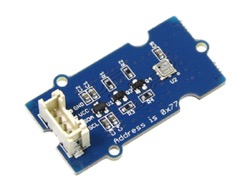
\includegraphics{../images/grovepi/barometer.jpg}
\caption{Barometer}
\end{figure}

\subsection{Distance Sensor}\label{distance-sensor}

Connect the distance sensor to a digital port. The grovepi module has a
built-in function to read the distance from the distance sensor, but it
is improperly calibrated, so this DistanceSensor class has a calibration
based on experimental data. The \texttt{DistanceSensor} class can be
found here:

\begin{itemize}
\tightlist
\item
  \href{https://github.com/cloudmesh/cloudmesh.pi/blob/master/cloudmesh/pi/distance.py}{DistanceSensor
  Class}
\end{itemize}

\begin{figure}
\centering

\includegraphics{../images/grovepi/distance.jpg}
\caption{Distance Sensor}
\end{figure}

\subsection{Temperature Sensor}\label{temperature-sensor}

The temperature sensor measures both temperature and humidity. Connect
the temperature sensor to a digital port. D7 is the default port. The
\texttt{TemperatureSensor} class can be found here:

\begin{itemize}
\tightlist
\item
  \href{https://github.com/cloudmesh/cloudmesh.pi/blob/master/cloudmesh/pi/temperature.py}{TemperatureSensor
  Class}
\end{itemize}

\begin{figure}
\centering
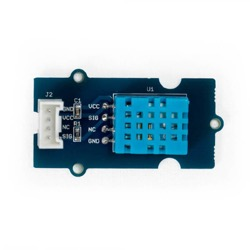
\includegraphics{../images/grovepi/temperature.jpg}
\caption{Temperature Sensor}
\end{figure}

\subsection{Heartbeat Sensor}\label{heartbeat-sensor}

Connect the heartbeat sensor to an I2C port. The heartbeat sensor
returns the heart rate of the wearer. The \texttt{HeartbeatSensor} class
can be found here:

\begin{itemize}
\tightlist
\item
  \href{https://github.com/cloudmesh/cloudmesh.pi/blob/master/cloudmesh/pi/heartbeat.py}{HearbeatSensor
  Class}
\end{itemize}

\begin{figure}
\centering
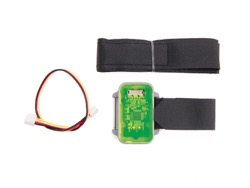
\includegraphics{../images/grovepi/heartbeat.jpg}
\caption{image}
\end{figure}

\subsection{Joystick}\label{joystick}

Connect the joystick to an analog port. A0 is the default port. The
joystick has an x, y, and click status based on the current state of the
module. The \texttt{Joystick} class can be found here:

\begin{itemize}
\tightlist
\item
  \href{https://github.com/cloudmesh/cloudmesh.pi/blob/master/cloudmesh/pi/joystick.py}{Joystick
  Class}
\end{itemize}

\begin{figure}
\centering
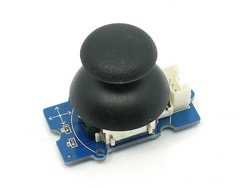
\includegraphics{../images/grovepi/joystick.jpg}
\caption{image}
\end{figure}

\subsection{LCD Screen}\label{lcd-screen}

The LCD screen can be used to display text and colors. In order to use
it, plug it into one of the I2C ports. The \texttt{LCD} class can be
found here:

\begin{itemize}
\tightlist
\item
  \href{https://github.com/cloudmesh/cloudmesh.pi/blob/master/cloudmesh/pi/lcd.py}{LCD
  Class}
\end{itemize}

\begin{figure}
\centering
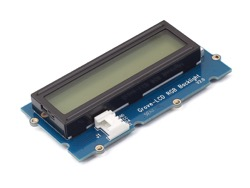
\includegraphics{../images/grovepi/lcd.jpg}
\caption{LCD Screen}
\end{figure}

\subsection{Moisture Sensor}\label{moisture-sensor}

Connect the moisture sensor to an analog port. The default port is A0.
The \texttt{MoistureSensor} class can be found here:

\begin{itemize}
\tightlist
\item
  \href{https://github.com/cloudmesh/cloudmesh.pi/blob/master/cloudmesh/pi/moisture.py}{MoistureSensor
  Class}
\end{itemize}

\begin{figure}
\centering
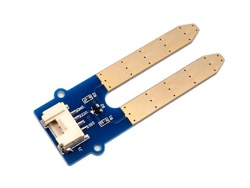
\includegraphics{../images/grovepi/moisture.jpg}
\caption{Moisture Sensor}
\end{figure}

An example of the implimentation of the moisture sensor from Dexter
Industries can be found
\href{https://github.com/DexterInd/GrovePi/blob/master/Projects/plant_monitor/plant_project.py}{here}.
The program is meant to measure the environmental conditions that affect
plant growth.

\subsection{Water Sensor}\label{water-sensor}

The water sensor measures the amount of water in the environment of the
sensor. Connect the sensor to a digital point. D2 is the default port.
The \texttt{WaterSensor} class can be found here:

\begin{itemize}
\tightlist
\item
  \href{https://github.com/cloudmesh/cloudmesh.pi/blob/master/cloudmesh/pi/water.py}{WaterSensor
  Class}
\end{itemize}

\begin{figure}
\centering
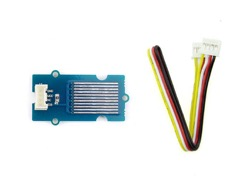
\includegraphics{../images/grovepi/water.jpg}
\caption{Water Sensor}
\end{figure}
